%basics of the document
\documentclass[12pt]{article}%font size and document style
\renewcommand{\baselinestretch}{1.5}%1.5 line spaceing
\usepackage{geometry}%marginals
\geometry{a4paper,
 left=35mm,
right=25mm,
 top=25mm,
bottom=25mm}
\setlength{\parindent}{0pt}%no indent on first line of paragraph

\usepackage{graphicx}%package for adding photos

\usepackage{eurosym}%euro symbol

\usepackage{wrapfig}%kuvien wrappaus

\usepackage{amsmath}%equation settings package

\usepackage{array}%package for editing table widths

\usepackage{xcolor}%different colors for text

\usepackage[linkbordercolor=white]{hyperref}%package for creating hyperinks

\usepackage{lipsum}%package for creating text

%biblatex bibtex reference package. Note that backend is biber not bibtex.
\usepackage[style=authoryear, maxbibnames=99, giveninits=true, dashed=False, backend=biber, minnames=1, maxcitenames=2]{biblatex}

%reference list settings
\DeclareNameAlias{sortname}{last-first}
\addbibresource{references.bib}%single bib file of all the references
\usepackage{xpatch,filecontents}
\xpatchbibmacro{date+extradate}{%no brackets around year
  \printtext[parens]%
}{%
  \setunit*{\space}%only space between name and last author
  \printtext%
}{}{} 
\makeatletter%no cursive
\renewrobustcmd*{\mkbibemph}{}
\protected\long\def\blx@imc@mkbibemph#1{#1}
\makeatother
\DeclareFieldFormat{pages}{#1}%no pp before pages
%no quetation marks on title of the reference
\DeclareFieldFormat[article]{title}{#1}
\DeclareFieldFormat[inproceedings]{title}{#1}
\DeclareFieldFormat[inbook]{title}{#1}
\renewbibmacro{in:}{}%no in
\AtEveryBibitem{\clearfield{number}}%no volyme number
\DeclareNameFormat{customauthor}{%custom author
  \namepartfamily
  \usebibmacro{name:andothers}}
%custom format for in book item
\DeclareBibliographyDriver{inbook}{%
  \printnames{author} 
  \printfield{year}%
  \newunit\newblock
  \printfield{title}%
  \newunit\newblock
  \printtext{In:}
  \printnames{editor}%
  \ifnumequal{\value{editor}}{1}
    {\printtext{\space(ed.)}}
    {\printtext{\space(eds.)}}
  \printfield{booktitle}%
  \newunit\newblock
  \printlist{publisher}%
  \printtext{,}
  \printlist{location}%
  \printtext{,}
  \printfield{pages}
  \finentry
}

%custom citation commands
%customformat i
\DeclareCiteCommand{\citei}
  {\usebibmacro{prenote}} 
  {\printnames[familyonly]{author}%
   \setunit{\addspace}%
   \ifnumgreater{\value{labelname}}{2}
     {\addspace et al.}
     {}%
   \printfield{year}%
   }
  {\multicitedelim}
  {\usebibmacro{postnote}}
%customformat ii
\DeclareCiteCommand{\citeii}
  {\usebibmacro{prenote}} 
  {\printnames[familyonly]{author}%
   \setunit{\addspace}%
   \ifnumgreater{\value{labelname}}{2}
     {\addspace et al.}
     {}%
   \printtext{(}%
   \printfield{year}%
   \printtext{)}
   }
  {\multicitedelim}
  {\usebibmacro{postnote}}

% custom name format 
\DeclareNameFormat{familyonly}{%
  \namepartfamily
  \ifnumgreater{\value{liststop}}{1}
    {\ifnumequal{\value{listcount}}{\value{liststop}}
      {}
      {\addspace and \addspace}}
    {}%
}

%pagenumber position
\usepackage{fancyhdr} % Custom headers and footers
\pagestyle{fancyplain} % Makes all pages in the document conform to the custom headers and footers
\fancyhead[L]{}% Empty left header
\fancyhead[C]{} % Page numbering for center header  
\fancyhead[R]{}% Empty right header
\fancyfoot[L]{}% Empty left footer
\fancyfoot[C]{}% Empty center footer
\fancyfoot[R]{}% Empty left footer
\renewcommand{\headrulewidth}{0pt}%no line


%add your own commands here
\newcommand{\aste}{^{\circ}}%command  for degree mark

\begin{document}
%%%%%%%%%%%%%%%%%%%%%%%%%%%%%%%%%%%%%%%%%%%%%%%%%%%%%%%%%%%%%%%%%%%%%%%%%%%%%%%%%%%%%%%%%%%%%%%%%%%%%%%%%%%%%%%%%%%%%%%%%%%%%%%%%%%%%%%%%%%%%%%%%%%%%%%%%%%%%%%%%%%%%%%%%%%%%%%%%%
\begin{titlepage}
\begin{center}
\vspace*{8cm}
Some info\\
\Large{\textbf{Title of the work}}\\
more info\\
\vspace*{4cm}
\tiny{You can also add photos or figures here.}
\end{center}
\end{titlepage}

%%%%%%%%%%%%%%%%%%%%%%%%%%%%%%%%%%%%%%%%%%%%%%%%%%%%%%%%%%%%
{\Large \textbf{Abstract}}\\
\lipsum[1]
\newpage

%%%%%%%%%%%%%%%%%%%%%%%%%%%%%%%%%%%%%%%%%%%%%%%%%%%%%%%%%%%%%%%%%%%%%%
\tableofcontents
\newpage

%%%%%%%%%%%%%%%%%%%%%%%%%%%%%%%%%%%%%%%%%%%%%%%%%%%%%%%%%%%%%%%%%%%%%%
%sivunumeroinnin aloits
\fancyhead[C]{\thepage}
\setcounter{page}{3}

\section{Tutorial}
I use program called TeXworks. It is availiable at least for Windws and Linux. I have no idea is online editors work if you just copy tex document to the editor.\\

Link to the github page of this file \href{https://github.com/Alekzanteri/hy_geo_latex}{github.com/Alekzanteri/hy\_geo\_latex}.

\subsection{References}
There is two custom cite commands that should follow graduopas. \textbackslash citei cretes citation such as "\citei{example1}" \textbackslash citeii creates citation "\citeii{example2}" 

\subsection{Figure example}
\begin{figure}[h]
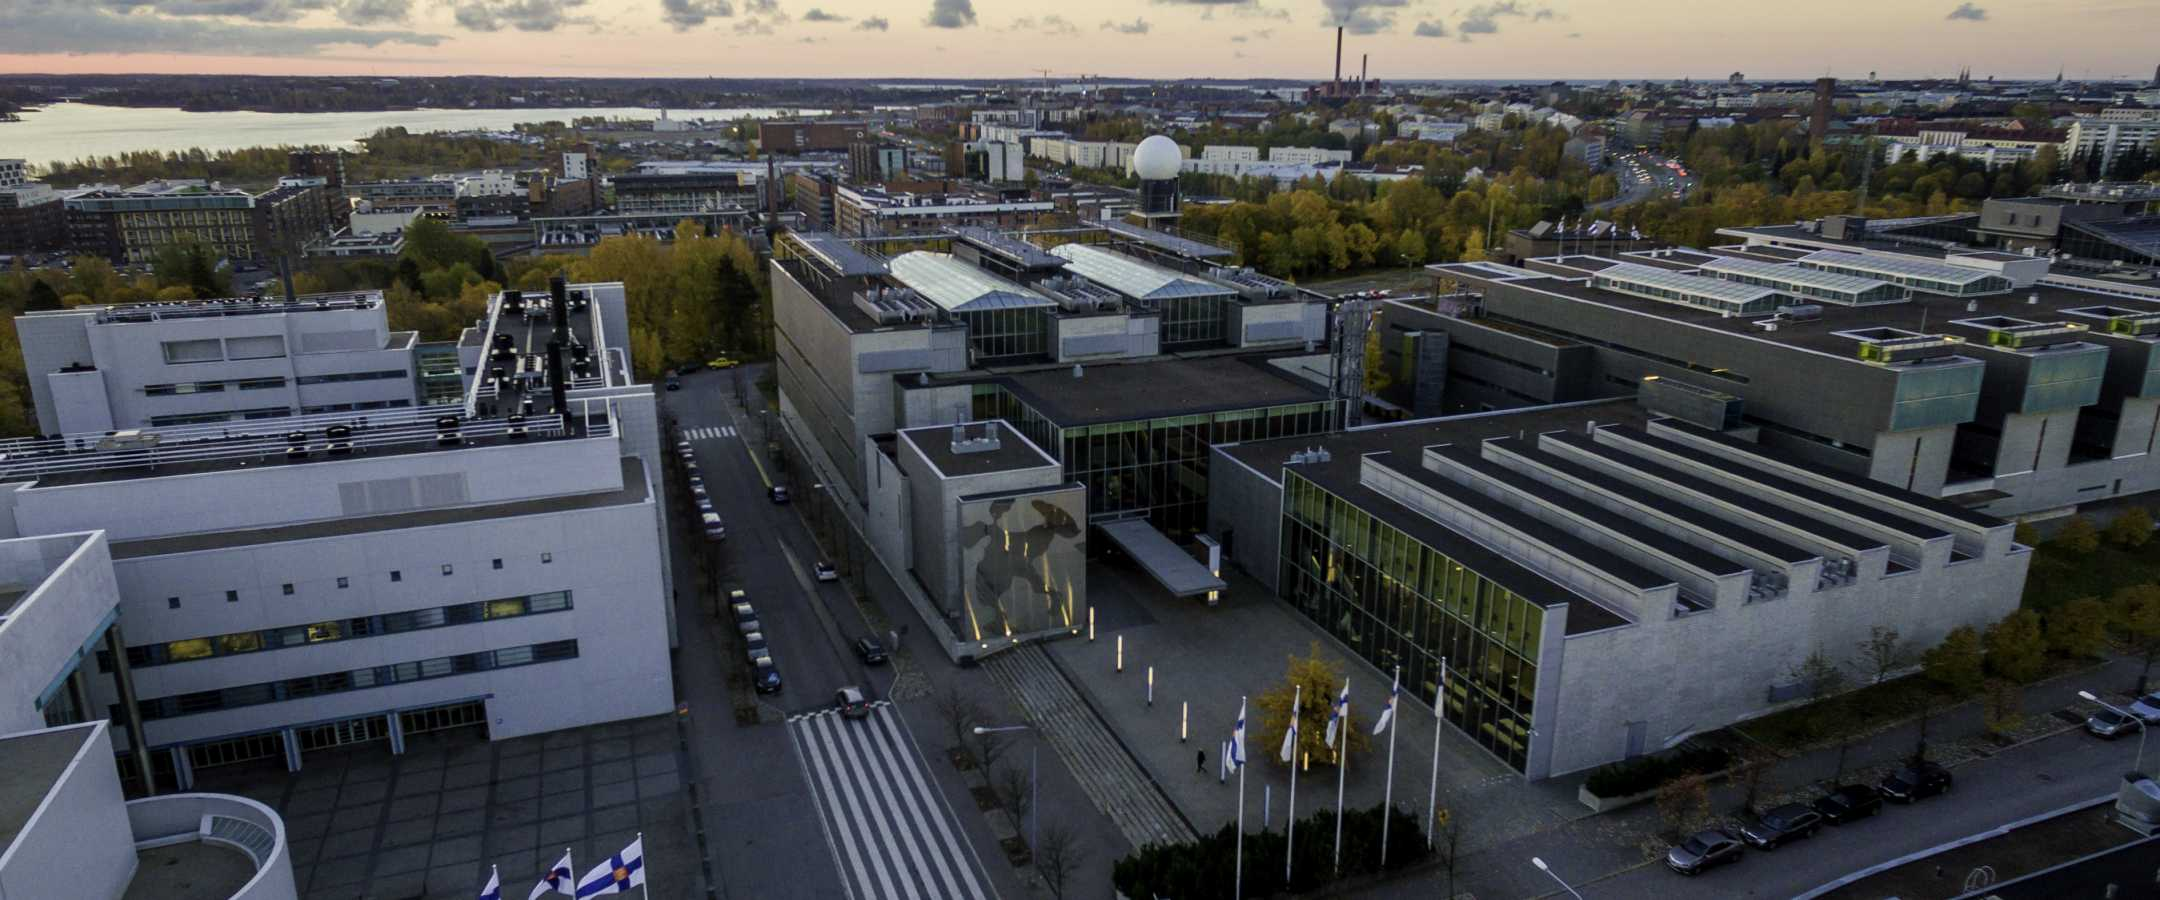
\includegraphics[width=\linewidth]{kumpula_ilmakuva.jpg}
\caption{Stolen photo of Kumpula campus.}
\end{figure}

\subsection{Math example}
\begin{equation}
\frac{420}{1312}\approx \frac13
\end{equation}

%%%%%%%%%%%%%%%%%%%%%%%%%%%%%%%%%%%%%%%%%%%%%%%%%%%%%%%%%%%%%%%%%%%%%%
\section{Lorem ipsunm}
\subsection{Do not read this}
\lipsum[1]

\subsection{or this}
\lipsum[1]

\subsection{they are both useless.}
\lipsum[1]

\section{References}
\printbibliography[title= \vspace{-1.5cm}]

%%%%%%%%%%%%%%%%%%%%%%%%%%%%%%%%%%%%%%%%%%%%%%%%%%%%%%%%%%%%%%%%%%%%%%%%%%%%%%%%%%%%%%%%%%%%%%%%%%%%%%%%%%%%%%%%%%%%%%%%%%%%%%%%%%%%%%%%%%%%%%%%%%%%%%%%%%%%%%%%%%%%%%%%%%%%%%%%%%%%%%%%%%%%%%%%%%%%%%%%%%%%%%%%%%
\end{document}